\section{Методология}

Целью работы было получить размеченный корпус и обученную модель, распознающую именованные сущности. После обзора литературы были намечены задачи и работа была предварительно разделена на несколько этапов.

\begin{enumerate}
\item Получение и разметка данных
\item Обучение и тюнинг моделей
\item Сравнение результатов
\end{enumerate}

Но в течение работы по нескольким причинам были внесены корректировки. Во-первых, как я упоминала ранее в обзоре литературы, с представленными результатами в статье Невзоровой невозможно сравниваться, поскольку цели моей и их работ различаются. Во-вторых, качество полученных данных оказалось не лучшим из возможных, а алгоритм Невзоровой, разработанный как раз для разметки данных, мог бы улучшить имеющийся корпус, используемый для обучения моделей. Как следствие, было принято решение воспроизвести алгоритм из статьи Невзоровой насколько это возможно и воспользоваться полученными результатами.

\begin{enumerate}
\item Получение и разметка данных
\item Обучение и тюнинг моделей
\item Воспроизведение статьи Невзоровой
\item Разметка данных с помощью алгоритма Невзоровой
\item Обучение и тюнинг моделей
\item Сравнение результатов
\end{enumerate}


\section{Получение и разметка данных}

\subsection{Туган Тел}

Обзор литературы показал, что существует корпус татарских текстов Туган Тел\cite{tugan_tel}. Данный копрус имеет также свою систему <<корпус-менеджер>>, которая представлена в виде сайта. На этом сайте можно искать по словоформе или лемме с огромным количеством параметров [\ref{fig:tugan_tel_1}], однако возможности просто скачать весь корпус не оказалось. Я предполагаю, что у Академии наук Республики Татарстан есть API для исполнения запросов на большом количестве данных и в каком-то более удобном формате, чем запрос на сайте, но у меня доступа к такому ресурсу нет. 

\begin{figure}
\caption{Параметры на сайте \href{http://tugantel.tatar/}{tugantel.tatar} для поиска по корпусу}
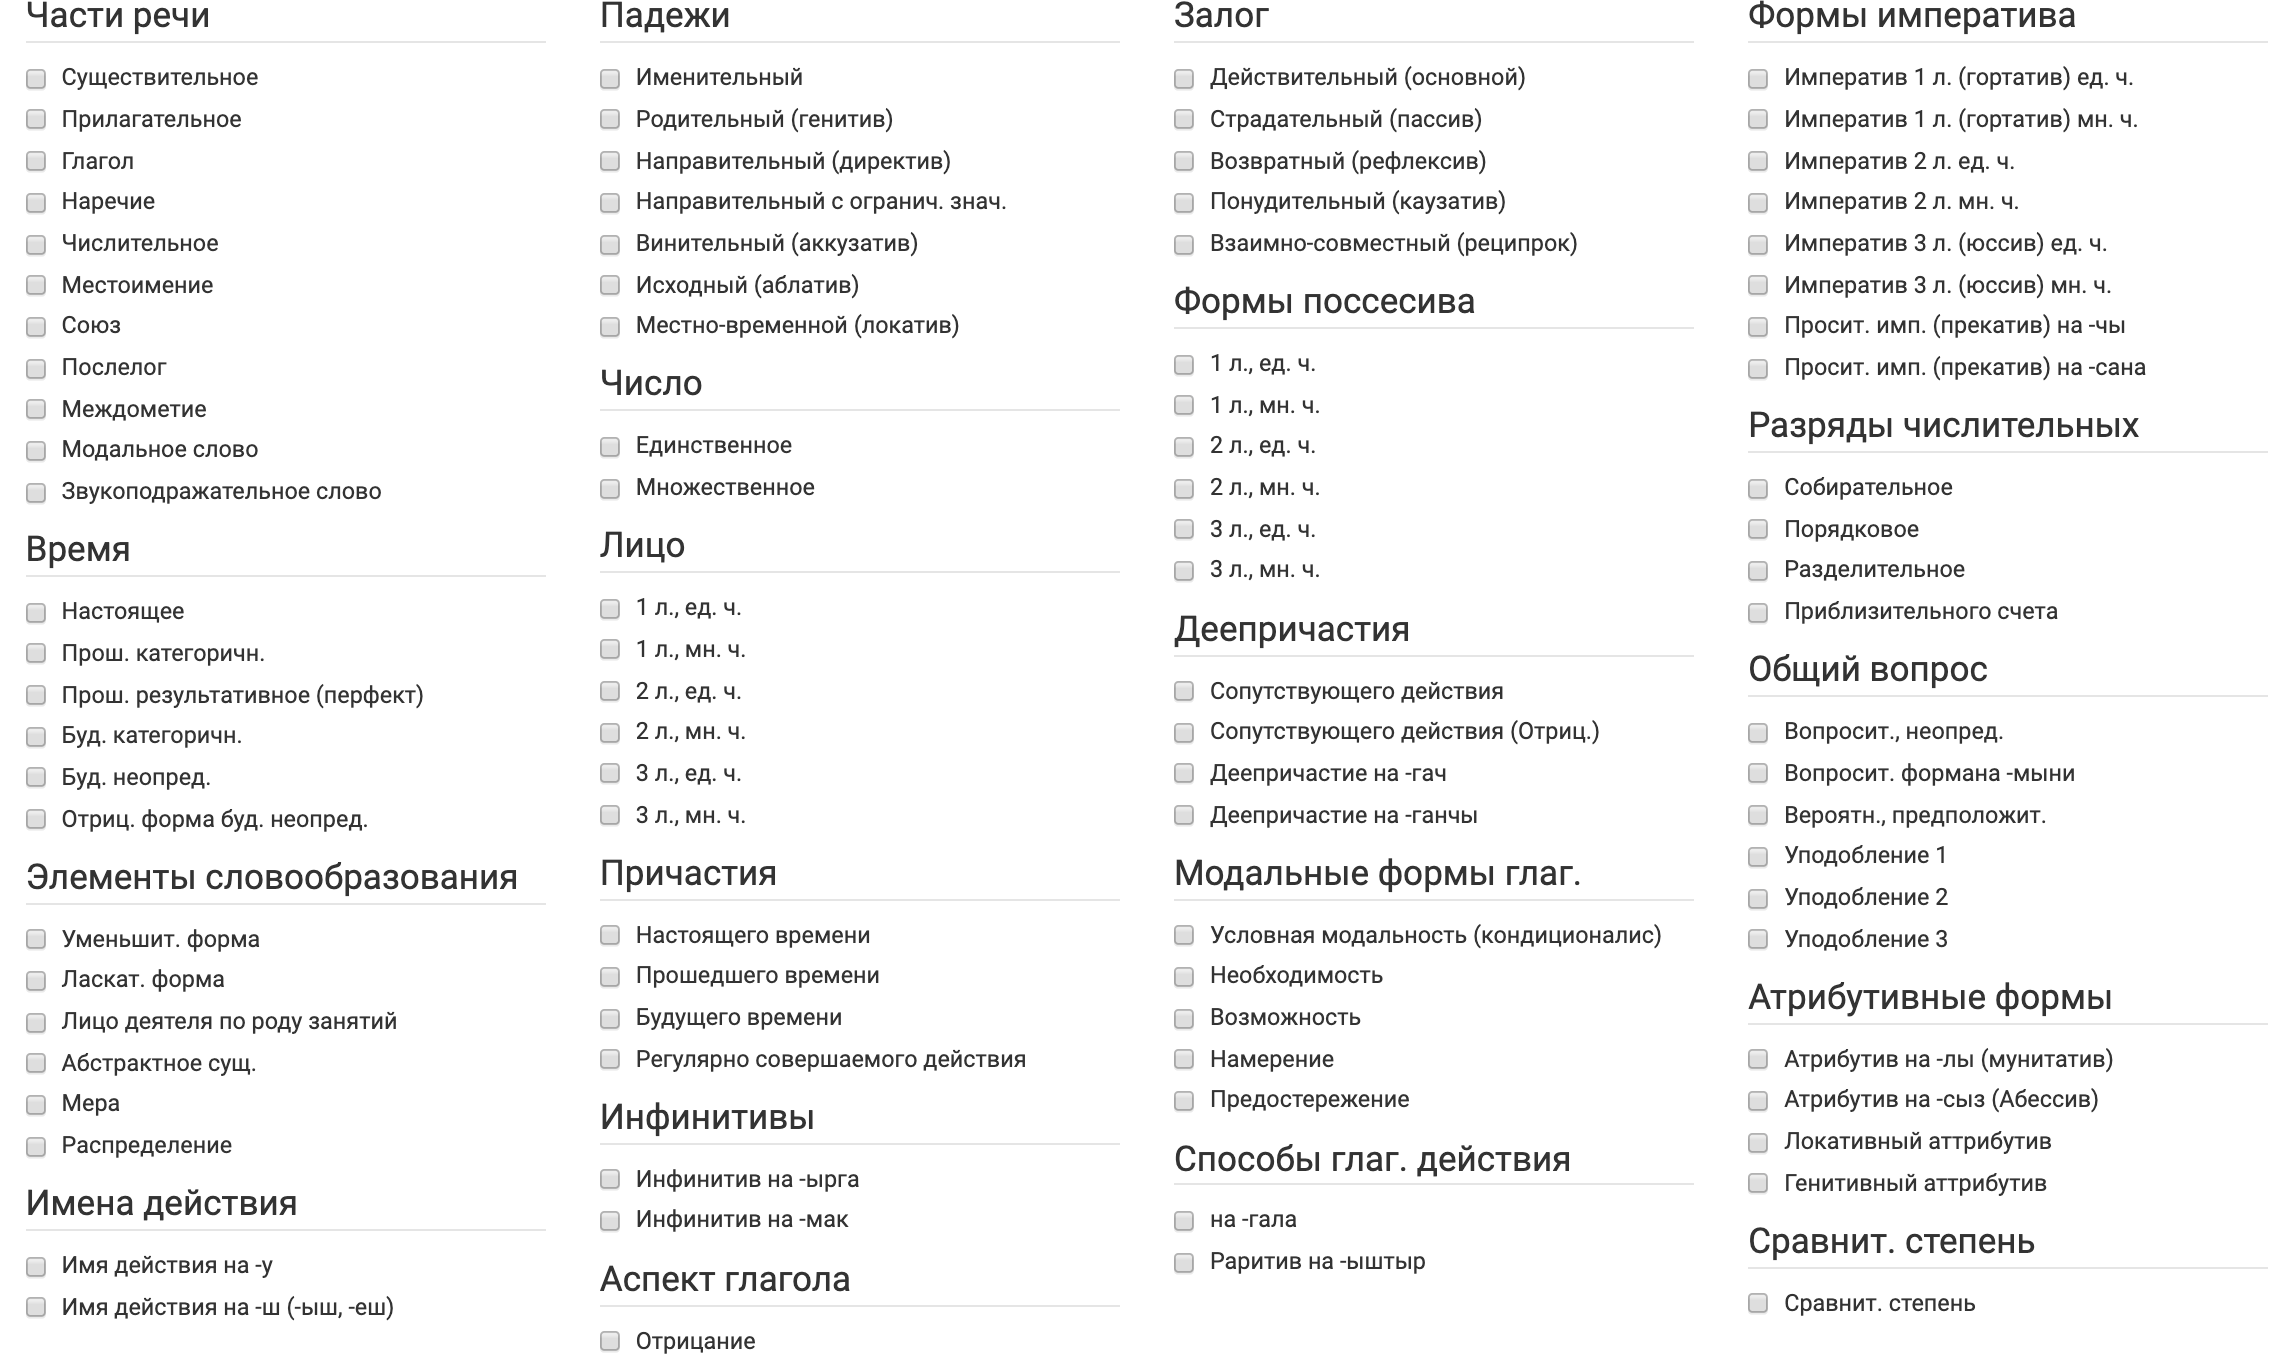
\includegraphics[width=\textwidth]{tugan_tel_1}
\label{fig:tugan_tel_1}
\end{figure}


Я связалась с Невзоровой по указанной в статье электронной почте, чтобы узнать подробности об их работе и попросить о сотрудничестве. Невзорова ответила на моё письмо и предоставила мне доступ к корпусу.

Корпус представляет из себя .zip файл, состоящий из $7557$ .txt файлов, в общей сложности весом $1\ 183\ 023\ 978$ Б. Как уже упоминалось ранее, корпус Туган Тел автоматически размечен с помощью программного инструментарии PC-KIMMO. Разметка выглядит следующим образом (см. рис \ref{fig:sample_sent}). На нечетной строке написано слово, на следующей --- разметка слова. Знаки препинания тоже являются <<словами>>.

\begin{figure}
\caption{Пример случайного предложения из корпуса Туган Тел}
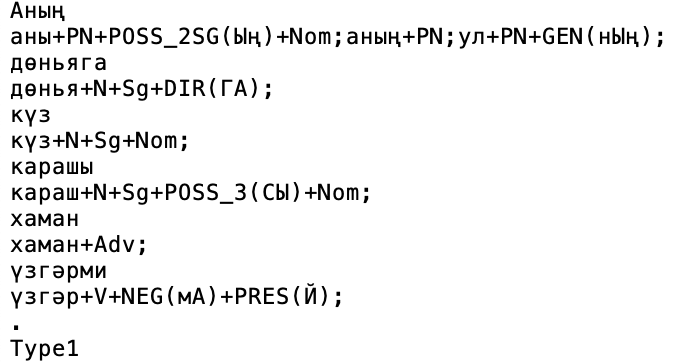
\includegraphics{sample_sent}
\label{fig:sample_sent}

Перевод: Его мировоззрение постоянно меняется.
\end{figure}

Поскольку я не использовала разметку никаким образом, кроме как для первой итерации выделения именованных сущностей, заострять внимание я не ней не буду.

\textcolor{red}{TODO} нужно ли вставлять описание тегов морфоанализатора?

В тегах морфоанализатора также присутствует тег PROP, который обозначает имя собственное. Сложно сказать, есть ли какая-то консистентность, но для первой итерации было решено применять этот тег в качестве именованной сущности. Как можно заметить в примере на рис. \ref{fig:prop_sent}, в корпусе имена собственные иногда бывают с маленькой буквы, что говорит о том, что данные содержат в том числе и ошибки.
Всего в текстах 30 753 824 слов, из них 534 514 это автоматически размеченные именованные сущности, что составляет $1,738\%$ от всех слов. 

\begin{figure}
\caption{Пример предложения из корпуса Туган Тел с атрибутом PROP}
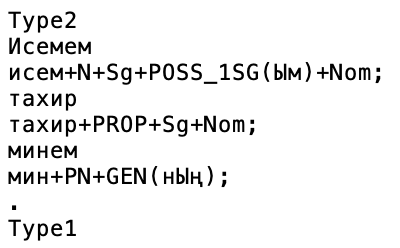
\includegraphics{pics/prop_sent}
\label{fig:prop_sent}

Перевод: Тахир меня зовут.
\end{figure}

\subsection{Татарская Википедия}

Кроме корпуса <<Туган Тел>> другого большого количества текстов, собранных в одном месте, найдено не было, поэтому было принято решение скачать википедию на татарском языке.

На данный момент татарская википедия содержит $89\ 252$ статей, которые написаны как с помощью кириллической, так и с помощью латинской письменности. Данный раздел Википедии был открыт 15 сентября 2003 года и сначала функционировал исключительно на латинице, позже статьи писались с использование обоих алфавитов; сейчас же достигнут консенсус об использовании единой системы категорий на кириллице, однако некоторые статьи до сих пор остаются латинизированными (примерно треть от всех имеющихся статей). Причин такой путаницы несколько. 

Во-первых, проблема алфавита в татарском языке стояла ещё со времен Советского Союза, т.к. до 1927 года использовалась арабская письменность, с 1927-1939 --- латинская письменность, а 5 мая 1939 года Президиум Верховного Совета Татарской АССР принял указ <<О переводе татарской письменности с латинизированного алфавита на алфавит на основе русской график>> и начал использоваться кириллический алфавит. Поскольку переход на другую письменность происходил принудительно, до сих пор ведутся дебаты о возвращении на латинский алфавит. На текущий момент в республике Татарстан кириллица остаётся официальным алфавитом, однако стало допустимым использование латиницы и арабицы при обращении граждан в государственные органы и латиницы при транслитерации. Существует официальное соответствие данных трёх алфавитов.

Во-вторых, в 2000-x годах существовала проблема с записью текстов на компьютере, вызванная отсутствием букв дополнительной кириллицы в стандартных раскладках.

В связи с этим статьи на латинице пришлось конвертировать в кириллицу и в то же время случайно не перевести английские названия (например, ссылки). Данная процедура была проведена с помощью автоматического скрипта, поэтому возможны артефакты в виде, например, слова <<хттп>>.

\begin{figure}[H]
\begin{minipage}{\textwidth}
\caption{Статья <<Камский бассейновый округ>>}
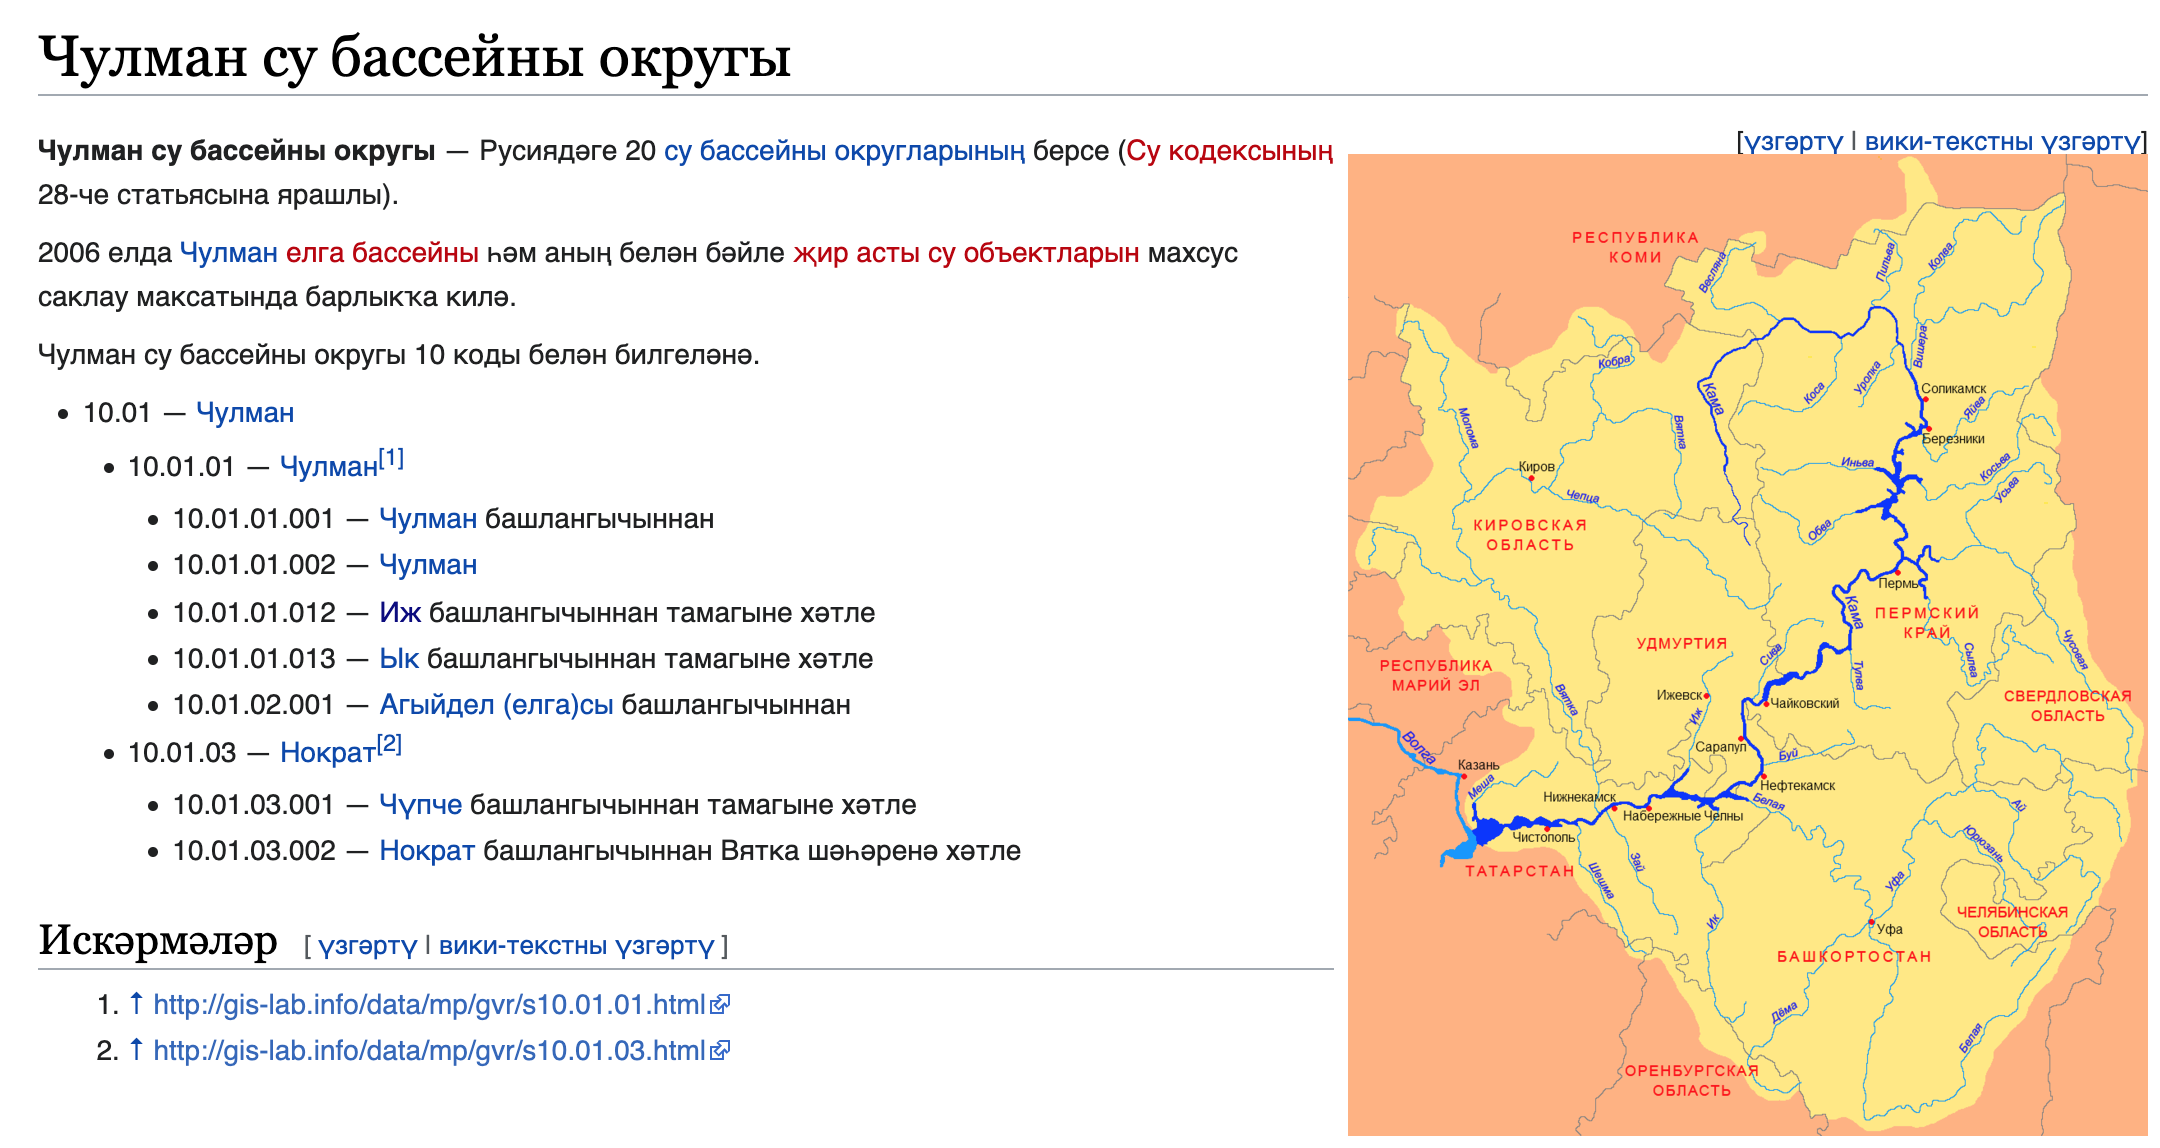
\includegraphics[width=\textwidth]{bassein_article}
\label{fig:bassein_article}
\end{minipage}

\begin{minipage}{\textwidth}
\caption{Пример сгенерированных статей из Википедии}
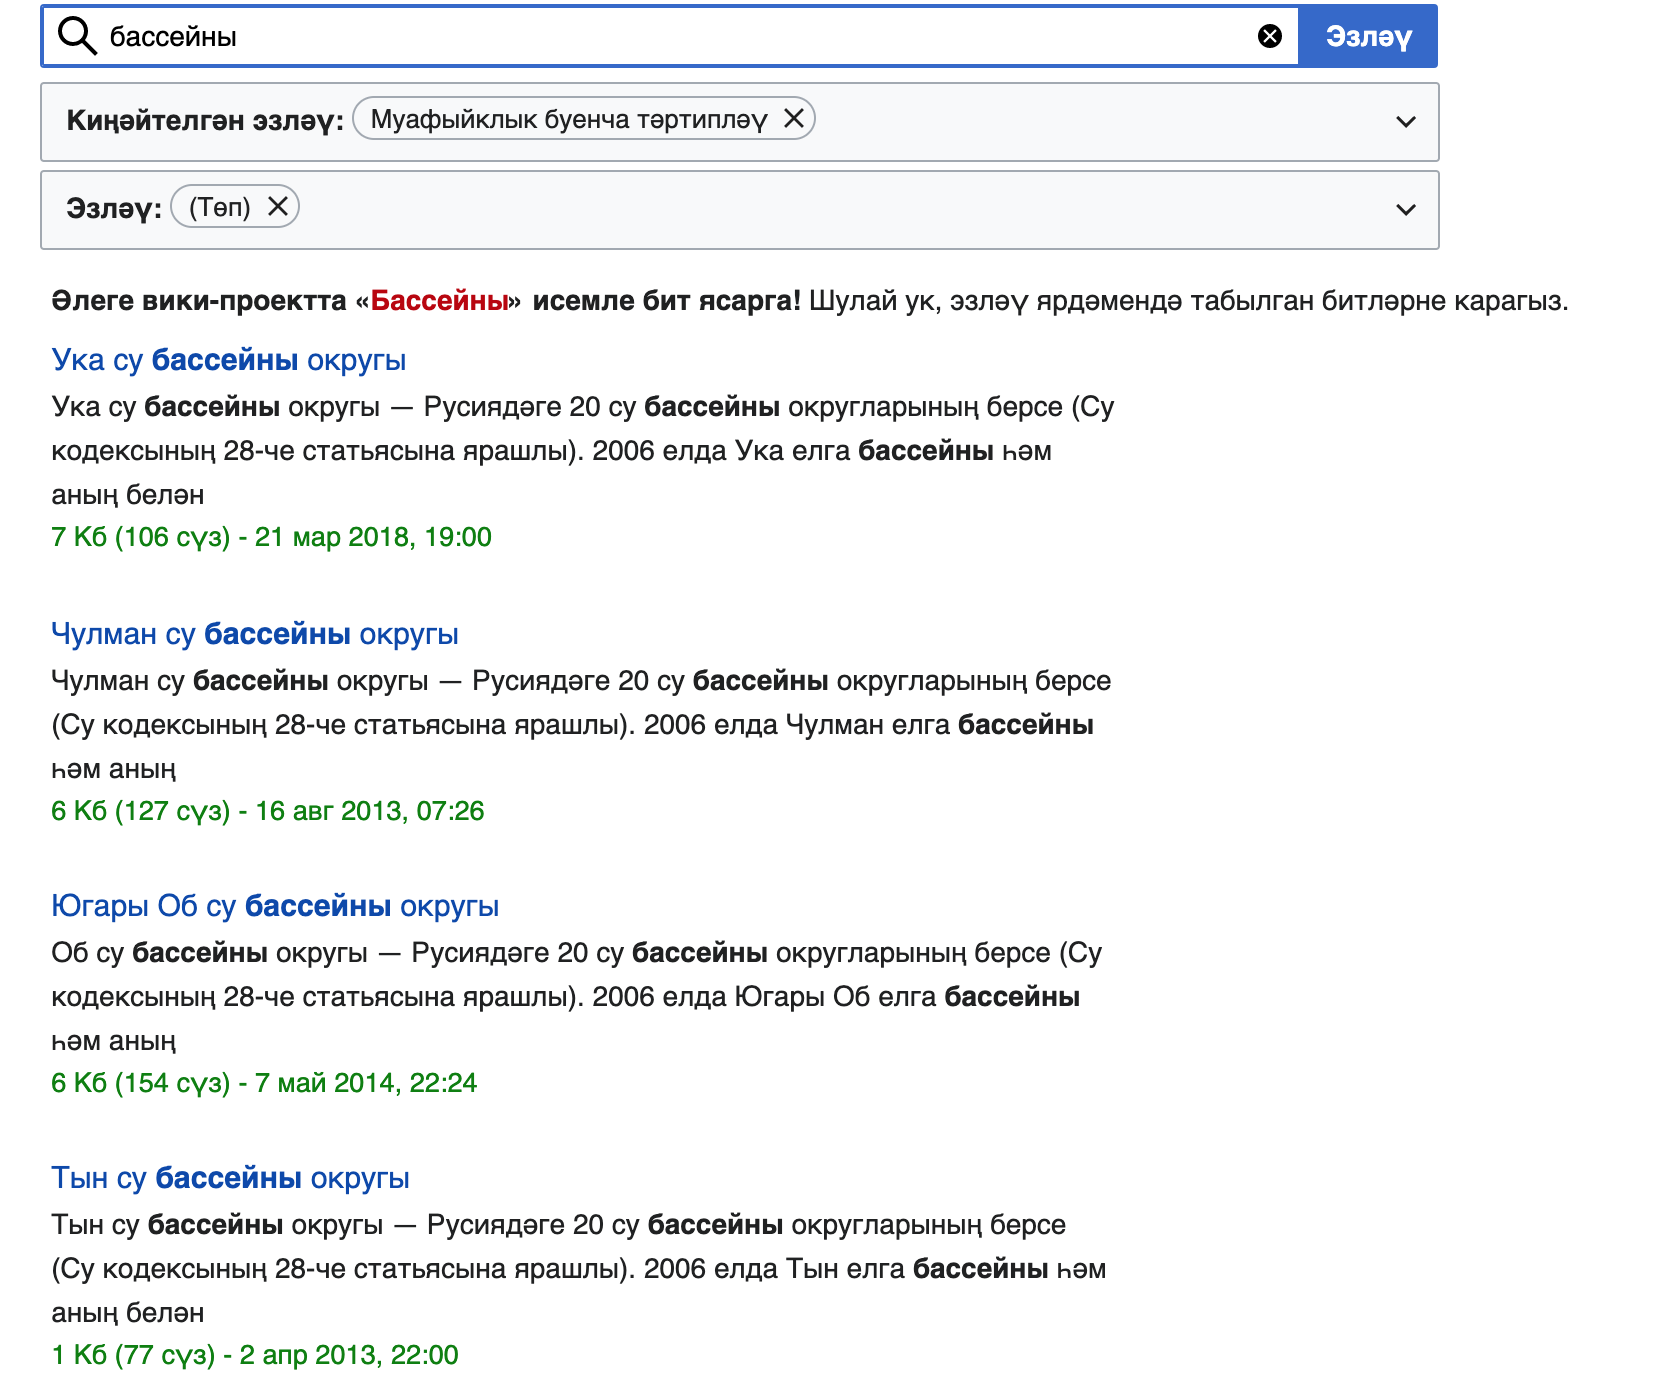
\includegraphics[width=\textwidth]{bassein_search}
\label{fig:bassein_search}
\end{minipage}
\end{figure}


Также важно отметить, что википедия представляет из себя набор статей, написанных в академическом стиле, что не вполне соответствует реальной человеческой речи; в этом аспекте Туган Тел гораздо лучше. В Википедии в том числе существуют автоматически сгенерированные статьи, это ухудшает качество текстов как корпуса для обучения, так как некоторые фразы становятся частотными не из-за того, что они действительно часто используются в языке, а из-за множества сгенерированных статей. Например, статьи про бассейновые округа (<<бассейны>> это не множественное число слова <<бассейн>>, а принадлежность к третьему лицу). Статья про Камский бассейновый округ (рис. \ref{fig:bassein_article}) и по тому же шаблону ещё много других статей про бассейновые округа (рис. \ref{fig:bassein_search}).

Справедливости ради, в русской википедии они тоже сгенерированы автоматически.

\subsection{Разметка данных для обучения}

Первой итерацией было использование разметки PROP в корпусе Туган Тел, никакие другие теги морфоанализотора не использовались; Википедия не использовалась. 

Во второй итерации использовался воспроизведенный алгоритм Невзоровой, в качестве <<данных>> для которого применялась Википедия. На данных из Википедии был получен список именованных сущностей по классам PER (персона), LOC (географический объект), ORG (организация) и MISC (всё остальное, но в основном названия языков) С помощью полученного списка была размечена Википедия, в то время как Туган Тел никак не использовался при данной разметке и был отложен в качестве данных для оценивания.

Для разметки BIO был написан небольшой скрипт, с помощью которого вы можете также получить размеченные данные на своей локальной машине.

\subsection{Разметка данных для оценивания}

Никакая автоматическая разметка не может быть настолько же идеальной, насколько ручная. Поэтому для оценивания воспроизведенного алгоритма Невзоровой и обученных моделей было принято решение разметить некоторое количество предложений самостоятельно, в силу имеющихся знаний татарского языка. Предложения выбирались из корпуса Туган Тел из соображений наличия в них хотя бы одной именованной сущности; для этого был использован алгоритм Невзоровой и если он определил наличие именованной сущности, то предложение добавлялось в список кандидатов на ручную разметку. Из полученного списка кандидатов предложения выбирались случайным образом, разметка алгоритмом Невзоровой удалялась до начала ручной разметки, чтобы не влиять на конечный результат. Получился датасет golden-bio.txt, основанный на предложениях из корпуса Туган Тел (~300 предложений).

\subsection{Проблемы с разметкой данных}

Как было описано и в статье Невзоровой, где исследователи глазами просматривали полученные результаты, отсеивали некорректные и улучшали свой алгоритм с помощью фильтров, так и в моей работе разметка данных происходила итеративно. Например, генерация статей в Википедии была как раз выявлена в просмотре полученных результатов после разметки. Также выявлялись пробелы в алгоритме, например, некоторые географические названия, которые не попадали в список, были добавлены позже вручную. Для разметки тегом PER был использован справочник имён. Подводя итог, лучшей всё равно остаётся ручная разметка, а любая автоматическая разметка требует просмотра и последующей корректировки, возможно в несколько этапов.

\section{Обучение и тюнинг моделей}

\subsection{BiLSTM-CRF}

Была использована модель BiLSTM-CRF из статьи <<A Neural Layered Model for Nested Named Entity Recognition>> \cite{ju-etal-2018-neural}. Она использует разметку BIO, как и многие другие модели для распознавания именованных сущностей. Архитектура модели изображена на рис. \ref{BiLSTMCRF}

\begin{figure}[H]
\caption{Архитектура модели BiLSTM-CRF, рис. из статьи \cite{ju-etal-2018-neural}}
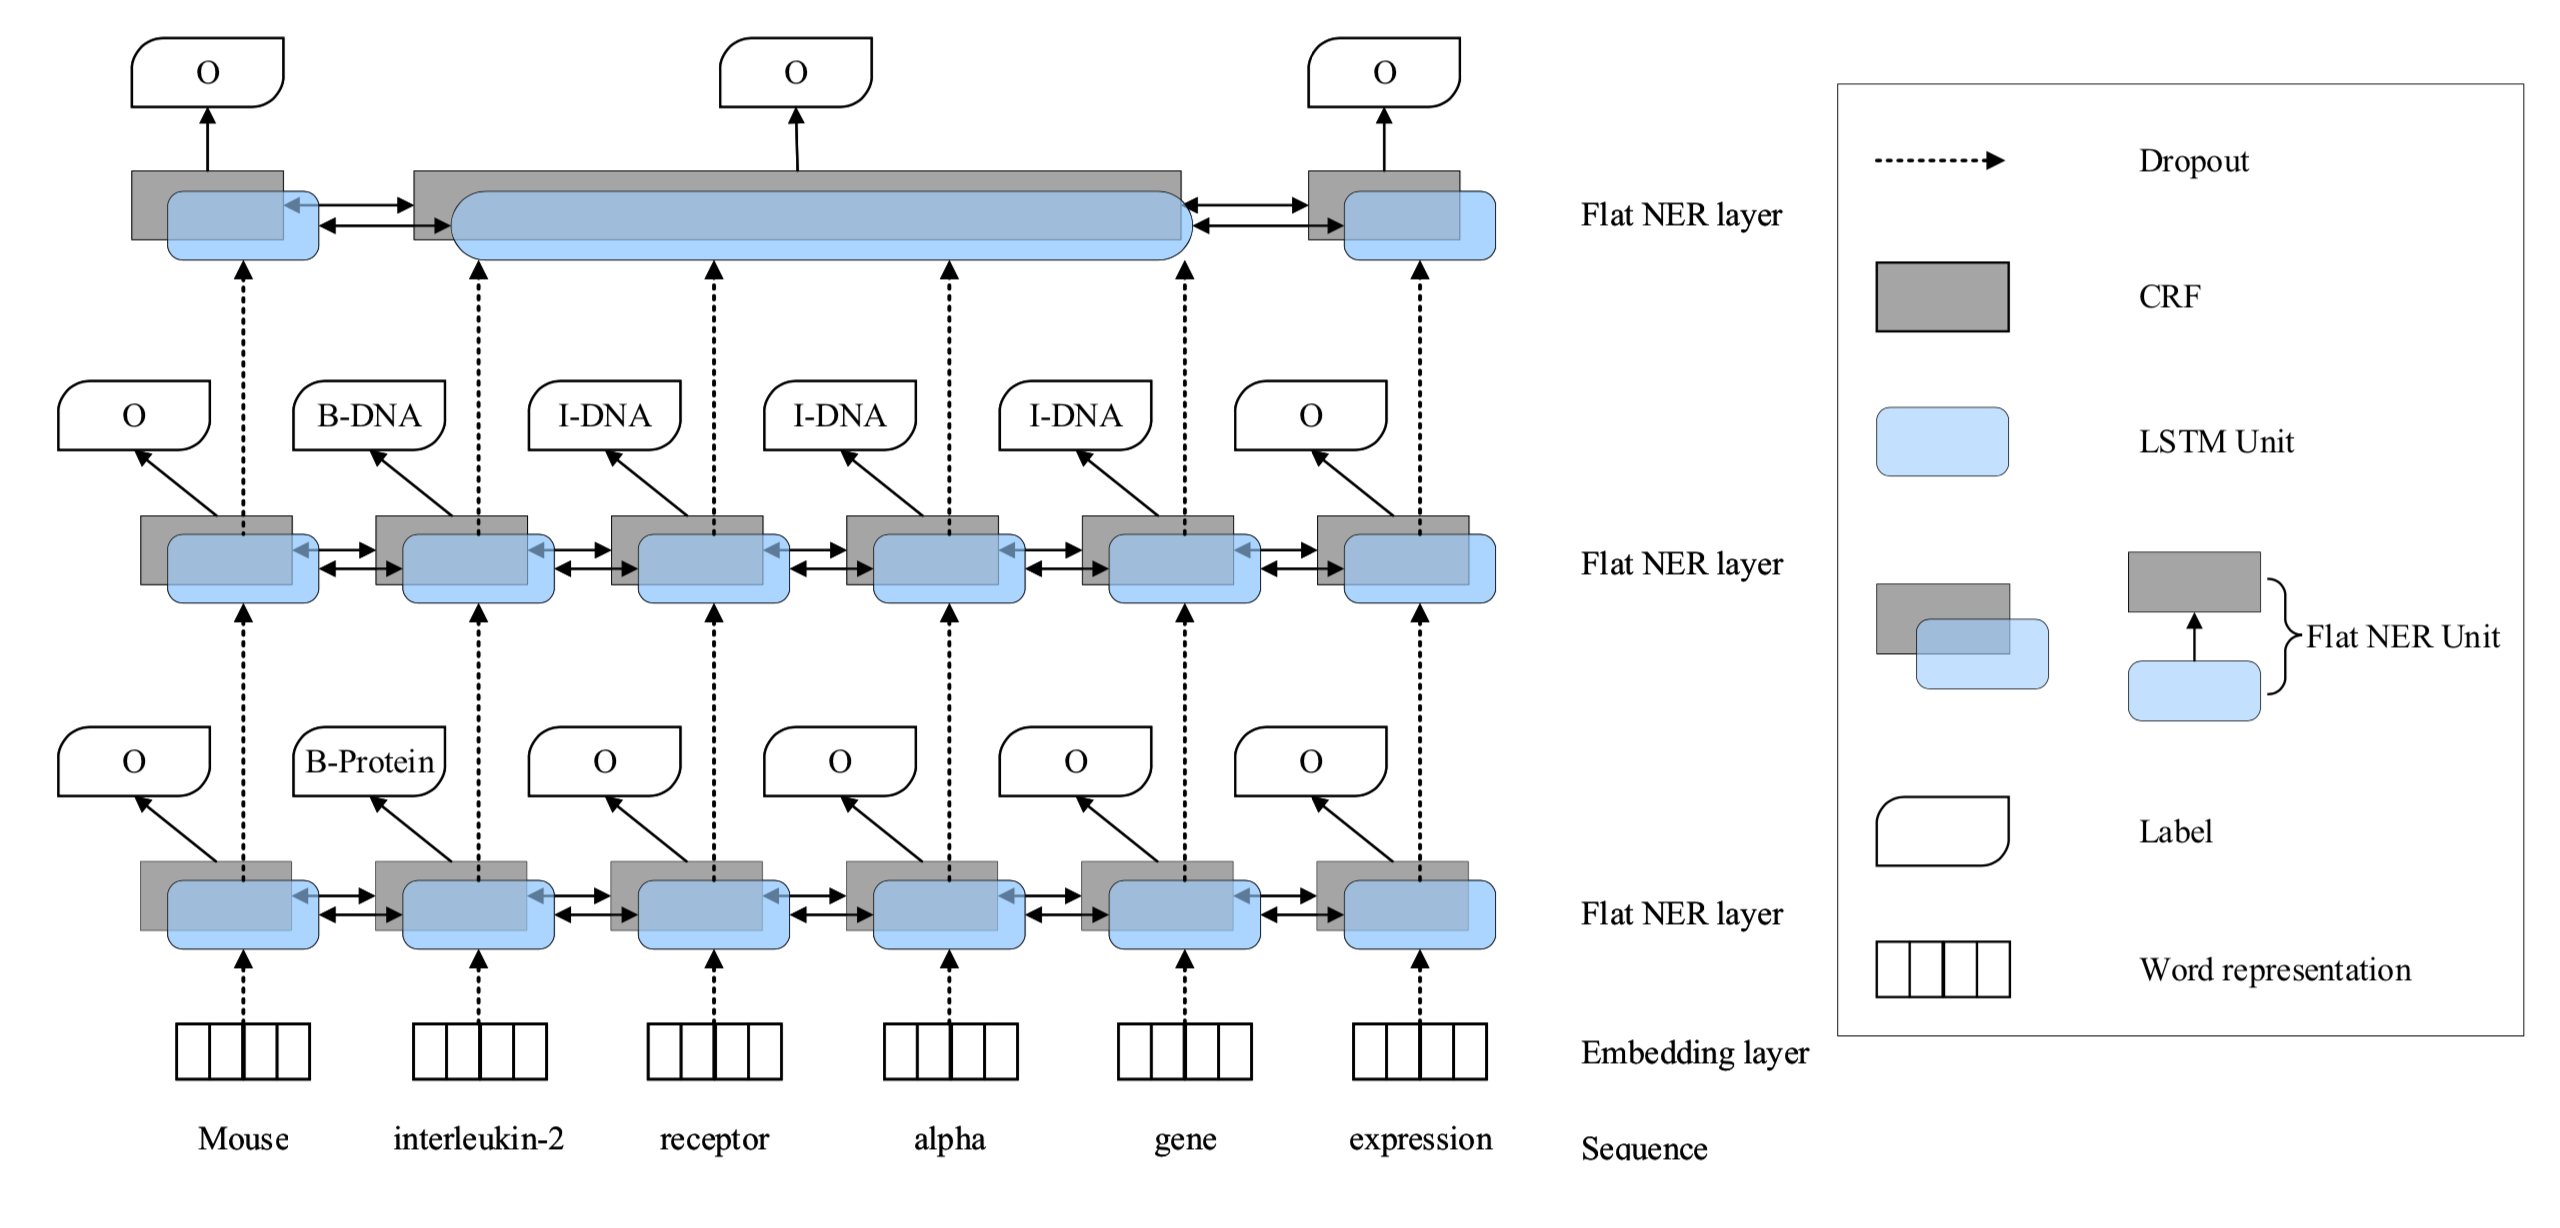
\includegraphics[width=\textwidth]{BiLSTMCRF}
\label{fig:BiLSTMCRF}
\end{figure}


Была возможность запустить модель только на локальной не очень мощной машине, поэтому пришлось обучаться не на всех данных, а только на части.

Первая итерация на данных Туган Тел, где тег PROP стал соответствовать тегу B-PER.

Результат обучения, в данных два тега: O и B-PER.

\textcolor{red}{TODO} Убрать последние 3 столбца?

\medskip

\begin{tabular}{| l | l | l | l | l | l | l |}
\hline
Category               & Precision  &   Recall   &  F-score   &  Predicts  &   Golds    &  Correct   \\

\hline
 PER                                 & 99.768     & 90.727     & 95.033     & 2589       & 2847       & 2583       \\
\hline
\end{tabular}


Была сделана демонстрация работы модели в виде сайта, запускающегося на локальной машине, но самые простые примеры не из тестового набора выявили большие несовершенства данной модели, поэтому в итоге было принято решение в целом отказаться от её использования. Как можно понять, цифры выше показывают возможность модели обучаться на данных (и модель действительно обучается хорошо, выборка разделяется на тестовую и валидационную и всегда показывает хороший результат), но проблема в том, что сами данные очень низкого качества --- и эту проблему модель, увы, исправить не может.


Далее сегодня я обучу модель на размеченной с помощью алгоритма Невзоровой Википедии и можно будет сравниться со всеми остальными моделями.


\subsection{BERT}

\cite{DBLP:journals/corr/abs-1810-04805} Одна из самых известных моделей на сегодняшний день, показала лучшие результаты на классических данных CoNLL 2003 (см. обзор литературы).

Для решения моей задачи была использована библиотека Hugging face \cite{Wolf2019HuggingFacesTS} и претренированная модель bert-base-multilingual-cased, которая обучена на чувствительных к регистру данных из 104-х наибольших Википедий. Данная модель включает в себя и татарский язык (беглый взгляд по токенам показал, что действительно есть как и кириллические, так и латинские токены на татарском языке). 

Опять возникла проблема с тем, что корпус слишком большой (вот уж иронично, что язык считается малоресурсным), но не с тем, что локальная машина не тянула обучение, а с тем, что библиотека torch использует библиотеку pickle для сохранения признаков, а библиотека pickle не сохраняет данных больше, чем на 4GB, а у меня, по моим прикидкам, признаков должно было получится на 13GB. В итоге пришлось ограничиться $1/3$ от всех данных. 

Первая итерация на данных Туган Тел, где тег PROP стал соответствовать тегу B-PER.

Результат обучения, в данных два тега: O и B-PER.

\medskip

\begin{tabular}{| l | l | l | l |}
\hline
Category               & Precision  &   Recall   &  F-score     \\

\hline
 PER                                 & 97.447     & 94.585    & 95.995        \\
\hline
\end{tabular}

Один в один повторение истории с BiLSTM-CRF --- сами по себе цифры очень многообещающие, модель обучилась прекрасно, но на деле они показывают всего лишь затренированность модели на плохих начальных данных, которая в итоге не работает на простых примерах, придуманных из головы. Было принято решение от этой модели отказаться.

Вторая итерация была на википедии, размеченной с помощью списка именованных сущностей, полученных с помощью алгоритма Невзоровой. В корпусе википедии были оставлены только те предложения, где есть хотя бы одна именованная сущность. 

\section{Воспроизведение статьи Невзоровой}

Была воспроизведена статья Невзоровой, на министерствах действительно показала хорошие результаты, но стало очевидно, что это полуручная история, потому что мусор пришлось выкидывать в ручном режиме. Ну и не удалось воспроизвести запросы в Туган Тел, а поиск был возможен только по слову (фразе). С помощью этого результата хочется разметить википедию, на википедии обучиться, а потом попытаться протестировать на Туган Тел и сравнить результаты.

\section{Сравнение результатов}

В процессе.


